
%(BEGIN_QUESTION)
% Copyright 2010, Tony R. Kuphaldt, released under the Creative Commons Attribution License (v 1.0)
% This means you may do almost anything with this work of mine, so long as you give me proper credit

This clearwell water level control system for a drinking water treatment facility maintains a constant level of water following filtration, for sourcing to customers:

$$\includegraphics[width=15.5cm]{i04509x01.eps}$$

Determine what both controllers (LIC and FIC) will do over time if the flow transmitter fails in such a way that it registers zero flow regardless of the actual flow rate of water through it.  Assume the level transmitter is direct-acting (i.e. greater signal with greater water level) and that the control valve is signal-to-open (fail closed).

\underbar{file i04509}
%(END_QUESTION)





%(BEGIN_ANSWER)

The flow controller (FIC) will send a ``full-open'' signal to the valve, because its transmitter indicates the flow rate is less than it should be. 

\vskip 10pt

The level controller's output will saturate low, telling the flow controller to stop the flow as the clearwell level rises well above setpoint due to the uncontrolled flow coming in. 

%(END_ANSWER)





%(BEGIN_NOTES)


%INDEX% Control, strategies: cascade

%(END_NOTES)


